\lecture{1}{26. Januar 2026}{Electrostatics}

\subsection{Coulomb's Law} \label{sec:coulomblaw}
\begin{equation*}
  \Vec{F} = k \frac{q_1 q_2}{r^2}\,\hat{r}
.\end{equation*}

\begin{assumptions}
  \item Point charges
\end{assumptions}

\begin{symbols}
  \InsertSym{estatfor}
  \InsertSym{coucon}
  \InsertSym{q1q2}
  \InsertSym{r}
  \InsertSym{rhat}
\end{symbols}

\subsubsection{Principle of Superposition}
\begin{equation*}
  \Vec{F}_{1, \mathrm{net}} = \sum_{i = 1}^{n} \Vec{F}_{1i}
.\end{equation*}

\begin{symbols}
  \InsertSym{F1net}
  \InsertSym{F1i}
\end{symbols}

\subsection{Quantization of Charge}
\begin{equation*}
  q = \pm n \cdot e
.\end{equation*}

\begin{symbols}
  \InsertSym{q}
  \InsertSym{zz}
  \InsertSym{echar}
\end{symbols}

\subsection{Electric Field at a point}
\begin{equation*}
  \Vec{E}(x,y,z) = \frac{\Vec{F}(x,y,z)}{q_0}
.\end{equation*}

\begin{symbols}
  \InsertSym{Exyz}
  \InsertSym{Fxyz}
  \InsertSym{q0}
\end{symbols}

\subsubsection{Electric Field Produced by Point Charge}
\begin{align*}
  \Vec{E} &= \frac{1}{4 \pi \epsilon_0} \frac{q}{r^2} \hat{r} \\
  E &= \frac{1}{4 \pi \epsilon_0} \frac{\left| q \right|}{r^2}
.\end{align*}

\begin{symbols}
  \InsertSym{Estr}
  \InsertSym{percon}
  \InsertSym{q}
  \InsertSym{r}
  \InsertSym{rhat}
\end{symbols}


\subsubsection{Electric Field due to a Dipole along dipole axis}
\begin{equation*}
  E(z) = E_{(+)}(z) + E_{(-)}(z) = \frac{q}{4\pi \epsilon_0 z^2} \left( \frac{1}{1 - \frac{d^2}{2z}} - \frac{1}{1 + \frac{d^2}{2z}} \right) = \frac{q}{2\pi \epsilon_0 z^3} \left( \frac{d}{\left( 1 - \left( \frac{d}{2z} \right)^2 \right)^2} \right)
.\end{equation*}

\begin{symbols}
  \InsertSym{Estr}
  \sym{$E_{(+)}, E_{(-)}$}{Contribution to $E$ from the positive and negative part of the dipole}{\unit{\N\per\C}}
  \InsertSym{percon}
  \InsertSym{z}
  \InsertSym{d}
  \InsertSym{q}
\end{symbols}

\subsubsection{Electric Field due to a Dipole along Dipole axis at Long Distance}
\begin{equation*}
  E = \frac{1}{2\pi \epsilon_0} \frac{qd}{z^3} = \frac{1}{2 \pi \epsilon_0} \frac{p}{z^3}
.\end{equation*}

\begin{assumptions}
  \item $z \gg d$, i.e. the distance between charges is much smaller then the distance from the charges you are measuring (``normal'' case)
\end{assumptions}

\begin{symbols}
  \InsertSym{Estr}
  \InsertSym{percon}
  \sym{$z$}{Distance along dipole axis}{\unit{\m}}
  \InsertSym{d}
  \InsertSym{q}
  \InsertSym{p}
\end{symbols}

\subsubsection{Electric Field of a Charged Ring at Large Distance}
\begin{equation*}
  E = \frac{1}{4 \pi \epsilon_0} \frac{q}{z^2}
.\end{equation*}

\begin{assumptions}
  \item $z \gg R$, i.e. distance from the ring is much grater than the radius of the ring
\end{assumptions}

\begin{symbols}
  \InsertSym{Estr}
  \InsertSym{percon}
  \sym{$q$}{Size of charge in the ring}{\unit{\C}}
  \sym{$z$}{Distance perpendicular to the radius of the ring}{\unit{\m}}
\end{symbols}


\subsubsection{Electric Field of a Charged Disk}
\begin{equation*}
  E = \frac{\sigma}{2 \epsilon_0} \left( 1 - \frac{z}{\sqrt{z^2 + R^2}} \right)
.\end{equation*}

\begin{assumptions}
  \item Infinitesimally thin disk
\end{assumptions}

\begin{symbols}
  \InsertSym{Estr}
  \InsertSym{percon}
  \InsertSym{sigmasurcharden}
  \sym{$z$}{Distance perpendicular to the disk}{\unit{\m}}
  \sym{$R$}{radius of disk}{\unit{\m}}
\end{symbols}

\subsubsection{Electric field from an infinite sheet}
\begin{equation*}
  E = \frac{\sigma}{2 \epsilon_0}
.\end{equation*}

\begin{assumptions}
  \item Infinitesimally thin infinite sheet
\end{assumptions}

\begin{symbols}
  \InsertSym{Estr}
  \InsertSym{sigmasurcharden}
  \InsertSym{percon}
\end{symbols}

\subsubsection{Electric field of a Conducting Sphere}
\begin{equation*}
  E = \frac{1}{4 \pi \epsilon_0} \frac{q}{r^2} = k \frac{q}{r^2}
.\end{equation*}

\begin{assumptions}
  \item Positive electric charge $Q$ distributed uniformly throughout the volume of a conducting sphere.
  \item Spherical symmetry
  \item No charge enclosed in conductor
\end{assumptions}

\begin{symbols}
  \InsertSym{Estr}
  \InsertSym{percon}
  \InsertSym{q}
  \InsertSym{r}
  \InsertSym{coucon}
\end{symbols}

\begin{figure} [ht]
  \centering
  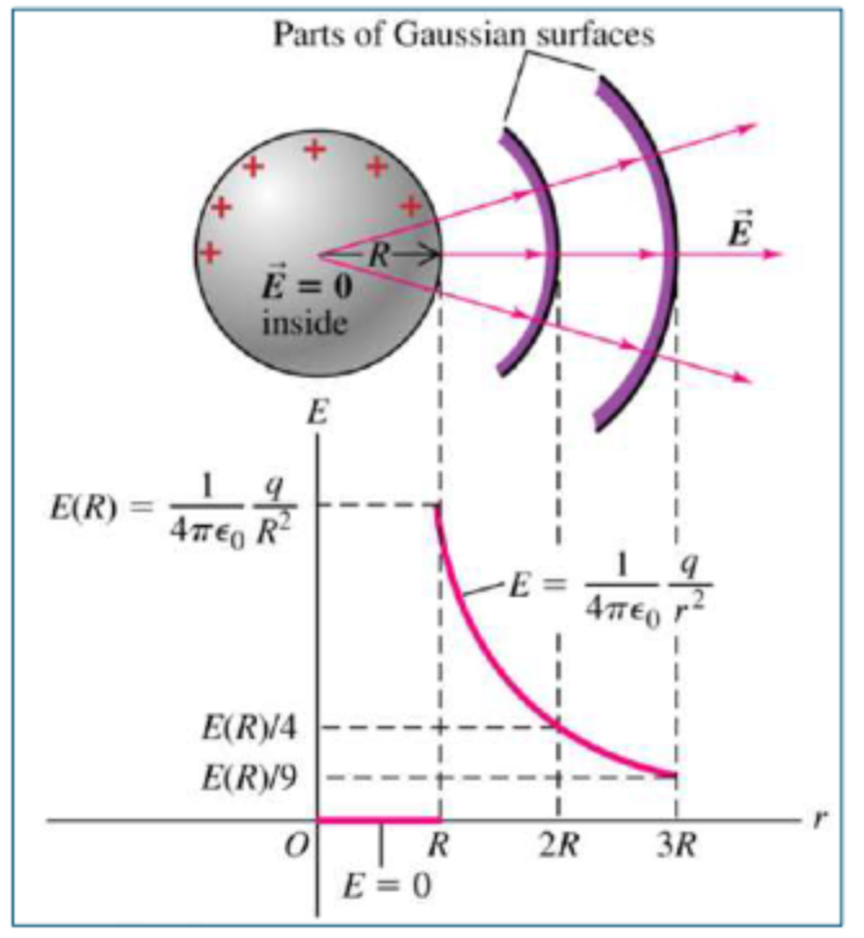
\includegraphics[width=0.5\linewidth]{./figures/econsph.png}
  \caption{E-field propagation from a conducting sphere.}
\end{figure}

\subsection{Electric Field of an Insulating Sphere}
\begin{align*}
  &\text{Outside}: & E &= \frac{1}{4\pi \epsilon_0} \frac{q}{r^2} \\
  &\text{Inside}: & E &= \frac{q}{4 \pi \epsilon_0 R^3} r
.\end{align*}

\begin{assumptions}
  \item Positive electric charge $Q$ distributed uniformly throughout the volume of an insulating sphere.
  \item Spherical symmetry
\end{assumptions}

\begin{symbols}
  \InsertSym{Estr}
  \InsertSym{r}
  \InsertSym{Rrad}
  \InsertSym{percon}
  \InsertSym{q}
\end{symbols}

\begin{figure} [ht]
  \centering
  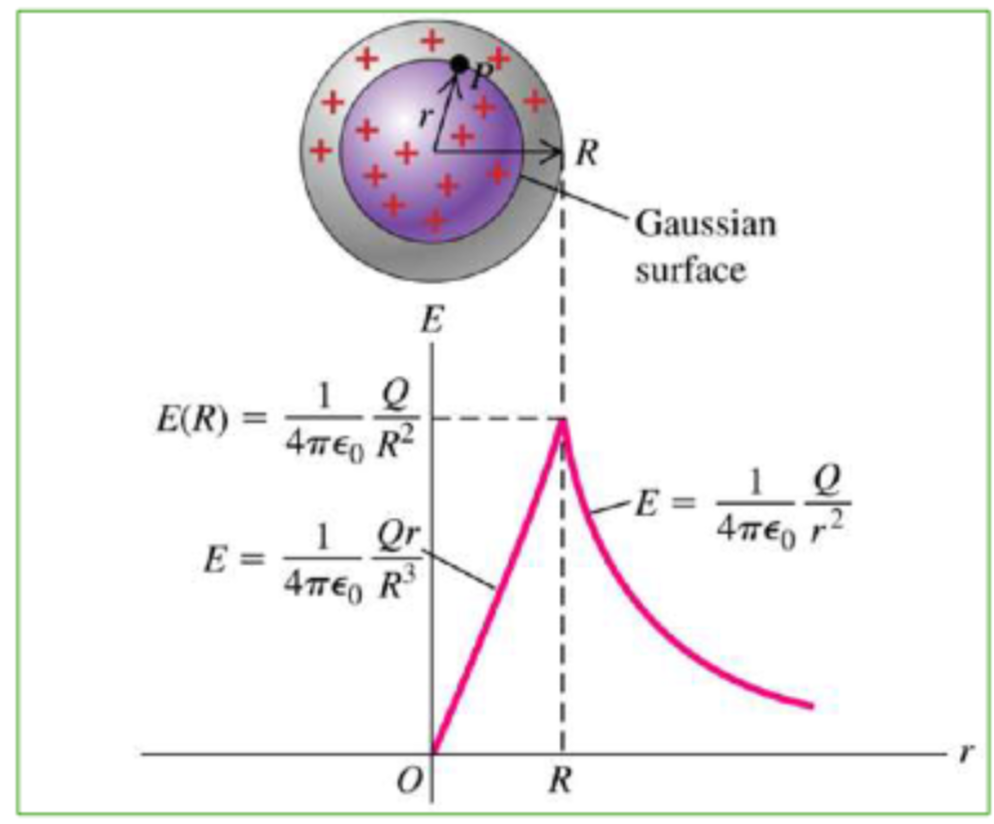
\includegraphics[width=0.5\linewidth]{./figures/einssph.png}
  \caption{E-field propagation through an insulating sphere.}
\end{figure}

\subsection{Gauss' Law}
\begin{equation*}
  \Phi = \frac{q_{\mathrm{enc}}}{\epsilon_0}
.\end{equation*}

\begin{assumptions}
  \item Vacuum (air)
\end{assumptions}

\begin{symbols}
  \InsertSym{Eflux}
  \InsertSym{qenc}
  \InsertSym{percon}
\end{symbols}

\subsubsection{Net electric flux through a surface caused by an electric field}
\begin{equation*}
  \Phi = \oint  \Vec{E} \cdot \mathrm{d}\Vec{A}
.\end{equation*}

\begin{symbols}
  \InsertSym{Eflux}
  \InsertSym{Evec}
  \InsertSym{Avec}
\end{symbols}

\subsection{Electric Potential Energy}

\begin{equation*}
  U_E = q_0 E \Delta d
.\end{equation*}

\begin{symbols}
  \InsertSym{UE}
  \InsertSym{q0}
  \InsertSym{Estr}
  \InsertSym{d}
\end{symbols}

\subsubsection{Electrostatic Potential}
\begin{equation*}
  V_E = \frac{U_E}{q_0}
.\end{equation*}

\begin{symbols}
  \InsertSym{VE}
  \InsertSym{UE}
  \InsertSym{q0}
\end{symbols}


\subsubsection{Electrostatic Potential of a Plate Capacitor}
\begin{equation*}
  V_E = E d
.\end{equation*}

\begin{symbols}
  \InsertSym{VE}
  \InsertSym{Estr}
  \InsertSym{d}
\end{symbols}
